\chapter{Εφαρμογές} % Main chapter title

\label{Chapter4} % Change X to a consecutive number; for referencing this chapter elsewhere, use \ref{ChapterX}

\section{Παραδείγματα εφαρμογών}
Το πρόβλημα εύρεσης του vertex cover ενός γράφου βρίσκει εφαρμογές σε διαφόρων ειδών προβλήματα τα οποία μπορεί εκ πρώτης όψεος να μην έχουν κάποιο κοινό γνώρισμα αλλά μπορούν να αναχθούν σε προβλήματα εύρεσης ενός ελαχίστου υποσύνολου το οποίο να "καλύπτει" ένα άλλο σύνολο.

\par{
Κάποια απλά παραδείγματα εφορμογής είναι τα εξής:

Έστω ότι θέλουμε να τοποθετήσουμε τροχονόμους στο οδικό δίκτυο μια πόλης, το πρόβλημα που προκύπτει είναι πώς μπορούμε να τοποθετήσουμε τους τροχονόμους με βέλτιστο τρόπο ώστε να χρησιμοποιήσουμε τον ελάχιστο αριθμό τροχονόμων που να "καλύπτουν" όλους τους δρόμους της πόλης. 
Αυτό το πρόβλημα μπορεί να μοντελοποιηθεί ως ένα minimum vertex cover πρόβλημα όπου οι ακμές είναι οι δρόμοι της πόλης και οι τροχονόμοι οι κόμβοι.
}
\par{
Άλλο παρόμοιο παράδειγμα: έστω ότι θέλουμε να τοποθετήσουμε κάμερες σε ένα κτήριο, πως μπορούμε να τοποθετήσουμε τις κάμερες με βέλτιστο τρόπο ώστε να έχουμε τον ελάχιστο αριθμό καμερών που να καλύπτουν όλους τους χώρους του κτηρίου; Και αυτό είναι ένα πρόβλημα που μπορεί να μοντελοποιηθεί ως minimum vertex cover πρόβλημα.
}

\par{
Ένα άλλο πρακτικό παράδειγμα είναι στην δυναμική ανίχνευση race conditions. Αν έχουμε ένα νήμα το οποίο γράφει σε μία θέσης μνήμης και έπειτα ένα άλλο νήμα προσπαθήσει να γράψει στην ίδια θέση μνήμης σημαίνει ότι κρατάει ένα lock για συγκεκριμένη θέση. Έτσι μπορούμε να ορίσουμε δύο σύνολα ένα το οποίο περιέχει τα νήματα και ένα που περιέχει τα locks για τις θέσεις μνήμης και ακμές που να αντιπροσωπεύουν την ιδιοκτησία κάποιου lock από ένα νήμα. Τότε το minimum hitting set αντιπροσωπεύει τον ελάχιστο σύνολο απο locks που είναι race-free. Το οποίο χρησιμοποιείται στη συνέχεια για την εξάλειψη περιττών εγγραφών.\cite{DataRaces}
}

\par{
Τέλος ένα παράδειγμα από τον τομέα της υπολογιστικής βιοχημείας όπου σε πολλά προβλήματα χρειάζεται η εξάλειψη συγκρούσεων μεταξύ αλληλουχιών ενός δείγματος. Το πρόβλημα μοντελοποείται ως γράφος όπου οι κόμβοι αντιπροσωπεύουν τις αλληλουχίες του δείγματος και οι ακμές τις μεταξύ τους συγκρούσεις. Ο στόχος είναι να αφαιρεθούν όσον το δυνατόν λιγότεροι κόμβοι ώστε να μην υπάρχουν καθόλου συγκρούσεις στον γράφο.\cite{SNP}
}

\section{Υλοποίηση}

{
\centering
\usemintedstyle{monokai}
\inputminted[
frame=lines,
framesep=2mm,
baselinestretch=1.2,
bgcolor=darkgray,
fontsize=\footnotesize,
linenos
]{cpp}{Figures/code.cpp}
}\\

\justify
Η παραπάνω συνάρτηση υλοποιεί τον προσεγγιστικό αλγόριθμο που παρουσιάστηκε στη παράγραφο 2.3.2. Η συνάρτηση καλείται σε ένα γράφο που αποτελείται από ένα σύνολο ακμών (edges) και ένα σύνολο κόμβων (vertices) και επιστρέφει ένα σύνολο κόμβων (vertex\_cover) που αντιπροσωπεύει το vertex cover του γράφου. Η συνάρτηση remove\_edge χρησιμοποιείται για να διαγράφει από ένα σύνολο ακμών όλες τις ακμές που είναι προσκύμενες σε ένα συγκεκριμένο κόμβο. Παρακάτω φαίνονται τα αποτελέσματα του αλγορίθμου, με κόκκινο συμβολίζονται οι κόμβοι που ανήκουν στο vertex cover του γράφου ενώ με άσπρο αυτοί που δεν ανήκουν.

\begin{figure}[H]
\caption{Vertex cover implementation example 1, 7 vertices}
\centering
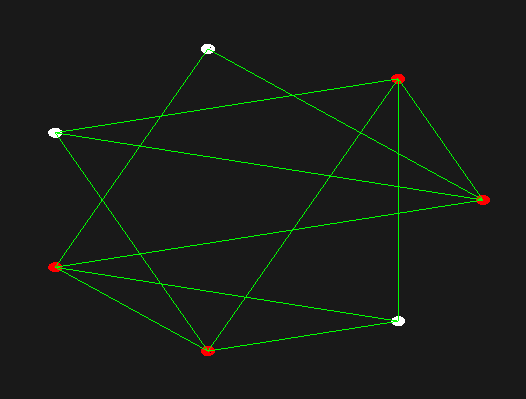
\includegraphics[width=0.6\textwidth]{Figures/code.png}\centering
\end{figure}

Με χρήση της βιβλιοθήκης Cbc που αποτελεί μέρος του COIN-OR project, και υλοποιεί αλγορίθμους για επίλυση προβλημάτων ακέραιου προγραμματισμού, μοντελοποιούμε το vertex cover problem σε πρόβλημα ακεραιού  προγραμματισμού. Φορτώνουμε τον πίνακα γειτνίασης του παραπάνω γράφου.

\begin{figure}[H]
\caption{Adjacency matrix}
\centering
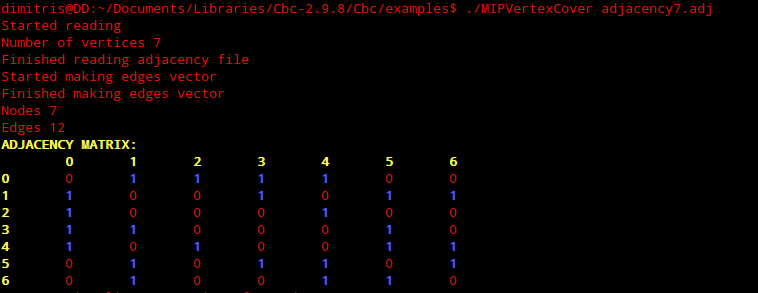
\includegraphics[width=1.1\textwidth]{Figures/adjac.png}\centering
\end{figure}

Και έπειτα τον χρησιμοποιούμε για να βρούμε τους περιορισμούς του προβλήματος.


\begin{figure}[H]
\caption{System Equations}
\centering
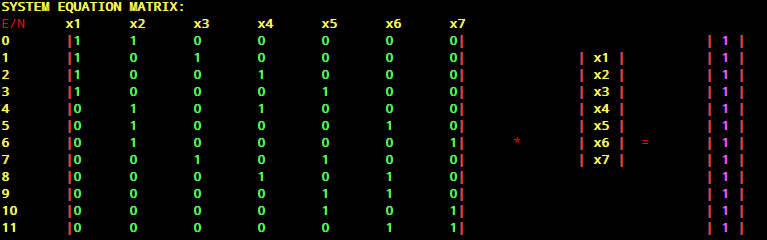
\includegraphics[width=1.1\textwidth]{Figures/sys.png}\centering
\end{figure}


\begin{figure}[H]
\caption{Solution}
\centering
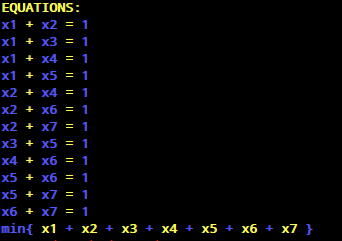
\includegraphics[width=0.6\textwidth]{Figures/const.png}\centering
\end{figure}

Και τέλος η λύση του προβλήματος δείχνει ότι επιλέγοντε 4 κόμβοι (αυτοί για τους οποίους η τιμή είναι 1) για το vertex cover όπως βρήκε και ο άπληστος αλγόριθμος.

\begin{figure}[H]
\caption{Vertex cover implementation example 1, 7 vertices}
\centering
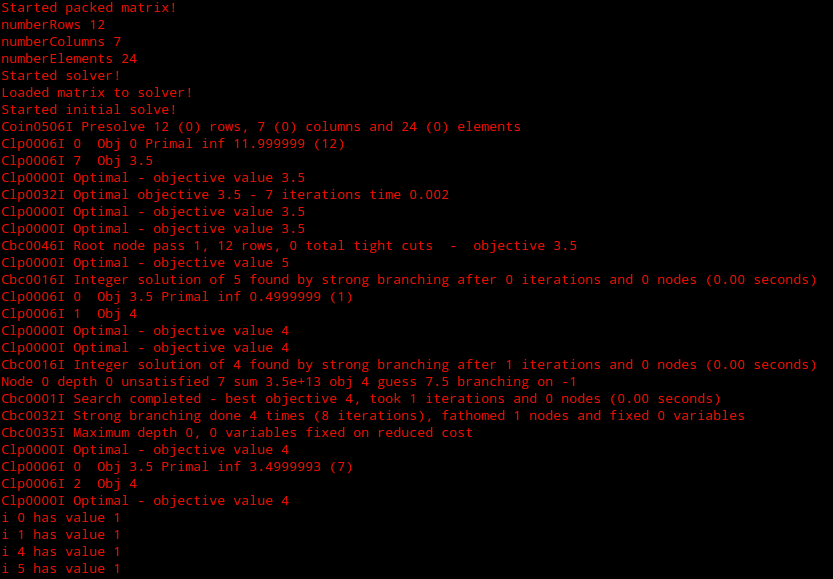
\includegraphics[width=1.3\textwidth]{Figures/sol_int.png}\centering
\end{figure}

Ενώ η χαλάρωση του προβλήματος και η λύση του με γραμμικό προγραμματισμό δίνει σε όλες τις μεταβλητές την τιμή 0.5, οπότε σύμφωνα με τα προηγούμενα θα πρέπει να επιλέξουμε όλους τους κόμβους στο vertex cover.

\begin{figure}[H]
\caption{Vertex cover implementation example 1, 7 vertices}
\centering
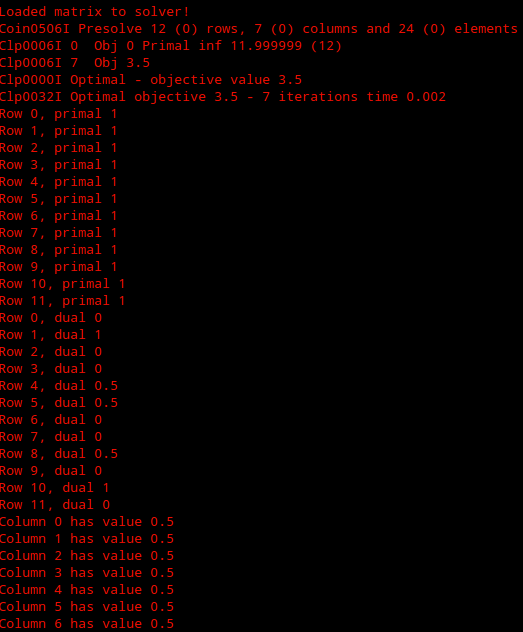
\includegraphics[width=1.1\textwidth]{Figures/sol_frac.png}\centering
\end{figure}